% \clearpage
% \appendix  % This command changes the section numbering to A, B, C...
% \addcontentsline{toc}{part}{Appendix}  % Add to main TOC as a part
% \part*{Appendix}  % Use \part* to avoid "Part I" numbering
% % \mtcaddchapter  % Tell minitoc this is a chapter-level entry
% \parttoc  % Generate the appendix TOC

% In your document where the appendix begins:
\clearpage
\appendix  % Switch to appendix mode (changes numbering to A, B, C...)

% Add appendix heading
\part*{Appendix}
\addcontentsline{toc}{part}{Appendix}  % Add to main TOC

% Create a local TOC for the appendix
\startcontents[appendix]
% \printcontents[appendix]{}{1}{\section*{Contents of Appendix}}
\printcontents[appendix]{}{1}{}

\section{Limitations}
\label{app:limitation}
Firstly, we mainly focus on math reasoning RL training that has the golden answer and support verifiable rewards. 
Tasks lacking verifiable rewards are not addressed in this manuscript.
Recent research~\cite{fu2025scaling} indicates that scaling reasoning may impair instruction-following capabilities, a challenge that can be alleviated by incorporating more comprehensive reward signals. 
% For instance, in open-ended generation tasks, the reward may be evaluated by an in-domain reward model.  
Secondly, we focus on 7B and smaller foundation models, due to the limited computational resources. Scaling LUFFY to larger models could be an interesting topic, given scaling law~\cite{scaling_law1,scaling_law2} is one of the most powerful principles in the area of large language models. 
Finally, as we are the first to incorporate off-policy guidance into the RLVR paradigm, we are limited to only including one off-policy trajectory per question, and find that one trajectory is already strong. However, extending off-policy guidance to multiple trajectories and multiple teachers could help the performance even further. 
% In addition, we 

\section{Theoretical Proof}
\label{app:theory}
\subsection{Convergence Rate of the Importance-Weighted Policy Gradient Estimator}
\label{app:convergence}

We study the nonconvex \emph{finite-sum} problems of the form
\begin{equation}
\max_{\bm{\theta}\in\mathbb{R}^d}J(\bm{\theta}) := \frac{1}{n}\sum_{i=1}^{n}J_i(\bm{\theta}),
\label{obj}
\end{equation}
where both $J$ and $J_i~(i\in[n])$ may be nonconvex.
We denote the class of such finite-sum Lipschitz smooth functions by $J\in\mathcal{J}_n$.
Here, we optimize functions in $\mathcal{J}_n$ of our importance-weighted policy gradient estimator. 

The vanilla policy gradient algorithm maximizes the expected advantage function (equivalent to minimizing the negative expected advantage function) as 
\begin{equation}
\max_{\bm{\theta}\in\mathbb{R}^d}J(\bm{\theta}) = \mathbb{E}_{\tau\sim\pi_{\bm{\theta}}}[A(\tau)]
\approx \frac{1}{n}\sum_{i=1}^{n}\left[A(\tau_i)\right],
\end{equation}

According to the Policy Gradient Theorem~\cite{sutton2018reinforcement}, the vanilla policy gradient estimator has the following form:
\begin{equation}
\nabla J(\bm{\theta}) = \mathbb{E}_{\tau\sim\pi_{\bm{\theta}}}\left[\nabla\log\pi_{\bm{\theta}}(\tau)\cdot A(\tau) \right]
\approx \frac{1}{n}\sum_{i=1}^{n}\left[\nabla\log\pi_{\bm{\theta}}(\tau_i)\cdot A(\tau_i)\right],
\end{equation}
where we use $\nabla J(\bm{\theta})$ to denote $\nabla_{\bm{\theta}} J(\bm{\theta})$ for simplicity. 
Our algorithm draws samples from another behavior policy $\pi_{\bm{\phi}}$, resulting in an importance-weighted policy gradient estimator as
\begin{equation}
\widetilde{\nabla} J(\bm{\theta}) = \mathbb{E}_{\tau\sim\pi_{\bm{\phi}}}\left[\frac{\pi_{\bm{\theta}}(\tau_i)}{\pi_{\bm{\phi}}(\tau_i)}\cdot\nabla\log\pi_{\bm{\theta}}(\tau)\cdot A(\tau) \right]
\approx \frac{1}{n}\sum_{i=1}^{n}\left[w_i\cdot \nabla J_i(\bm{\theta})\right],
\end{equation}
where $w_i=\frac{\pi_{\bm{\theta}}(\tau_i)}{\pi_{\bm{\phi}}(\tau_i)}$ is the importance weight assigned to sample $i$.


Let $\alpha_k$ denote the learning rate at iteration $k$, and $w_{i_k}$ be the instance weight assigned to sample $i$ by our algorithm.
By stochastic gradient ascent, our algorithm has the following update rule:
\begin{eqnarray}
\bm{\theta}^{k+1} = \bm{\theta}^k + \alpha_kw_{i_k}\nabla J_{i_k}(\bm{\theta}^k), i\in [n].
\label{iter}
\end{eqnarray}


\begin{definition}
For $J\in\mathcal{J}_n$, our algorithm takes an index $i\in[n]$ and a point $x\in\mathbb{R}^d$, and returns the pair $(J_i(\bm{\theta}),\nabla J_i(\bm{\theta}))$.
\end{definition}

\begin{definition}
We say $J:\mathbb{R}^d\to \mathbb{R}$ is Lipschitz smooth ($L$-smooth) if there is a constant $L$ such that
\begin{equation}
||\nabla J(\bm{\vartheta}) - \nabla J(\bm{\theta})||\le L||\bm{\vartheta}-\bm{\theta}||,~~~\forall \bm{\vartheta},\bm{\theta}\in \mathbb{R}^d.
\end{equation}
\end{definition}

\begin{definition}
A point $\bm{\theta}$ is called $\epsilon$-accurate if $||\nabla J(\bm{\theta})||^2\le\epsilon$.
A stochastic iterative algorithm is said to achieve $\epsilon$-accuracy in $k$ iterations if $\mathbb{E}[||\nabla J(\bm{\theta}^k)||^2\le \epsilon$, where the expectation is over the stochasticity of the algorithm.
\end{definition}

\begin{definition}
We say $J\in\mathcal{J}_n$ has $\sigma$-bounded gradients if $||\nabla J_i(\bm{\theta})||\le\sigma$ for all $i\in[n]$ and $\bm{\theta}\in\mathbb{R}^d$.
\label{bound}
\end{definition}


\begin{definition}
We say the positive instance weight $w$ in our algorithm is bounded if there exist constants $\underline{w}$ and $\overline{w}$ such that $\underline{w}\le w_i \le \overline{w}$ for all $i\in[n]$.
\label{iw}
\end{definition}


\setcounter{theorem}{0}
\begin{theorem}\label{thm:con_app}
Suppose the objective function of the policy gradient algorithm $J\in\mathcal{J}_n$, where $\mathcal{J}_n$ is the class of finite-sum Lipschitz smooth functions, has $\sigma$-bounded gradients, and the importance weight $w=\pi_{\bm{\theta}}/\pi_{\bm{\phi}}$ is clipped to be bounded by $[\underline{w}, \overline{w}]$.
Let $\alpha_k=\alpha=c/\sqrt{K}$ where $c = \sqrt{\frac{2(J(\bm{\theta}^*)-J(\bm{\theta}^0))}{L\sigma^2\underline{w}\overline{w}}}$, and $\bm{\theta}^*$ is an optimal solution. 
Then, the iterates of our algorithm in Eq.~(\ref{iw_pg}) satisfy:
\begin{eqnarray}
\min_{0\le k\le K-1}\mathbb{E}[||\nabla J(\bm{\theta}^k)||^2] \le \sqrt{\frac{2(J(\bm{\theta}^*)-J(\bm{\theta}^0))L\overline{w}}{K\underline{w}}}\sigma. \nonumber
\end{eqnarray}
\end{theorem}

\begin{proof}
According to the Lipschitz continuity of $\nabla J$, the iterates of our algorithm satisfy the following bound:
\begin{eqnarray}
\mathbb{E}[J(\bm{\theta}^{k+1})] \geq \mathbb{E}[J(\bm{\theta}^k) + \langle\nabla J(\bm{\theta}^k),\bm{\theta}^{k+1}-\bm{\theta}^k\rangle - \frac{L}{2}||\bm{\theta}^{k+1}-\bm{\theta}^k||^2].
\label{Lcon}
\end{eqnarray}
After substituting~(\ref{iter}) into~(\ref{Lcon}), we have:
\begin{eqnarray}
\mathbb{E}[J(\bm{\theta}^{k+1})] 
\!\!\!\!\!\!&& \geq \mathbb{E}[J(\bm{\theta}^k)] + \alpha_kw_k\mathbb{E}[||\nabla J(\bm{\theta}^k)||^2] - \frac{L\alpha_k^2w_k^2}{2}\mathbb{E}[||\nabla J_{i_k}(\bm{\theta}^k)||^2] \nonumber \\
\!\!\!\!\!\!&& \geq \mathbb{E}[J(\bm{\theta}^k)] + \alpha_kw_k\mathbb{E}[||\nabla J(\bm{\theta}^k)||^2] - \frac{L\alpha_k^2w_k^2}{2}\sigma^2. \label{f}
\end{eqnarray}
The first inequality follows from the unbiasedness of the stochastic gradient $\mathbb{E}_{i_t}[\nabla J_{i_k}(\bm{\theta}^k)]=\nabla J(\bm{\theta}^k)$.
The second inequality uses the assumption on gradient boundedness in Definition~\ref{bound}.
Re-arranging~(\ref{f}) we obtain
\begin{eqnarray}
\mathbb{E}[||\nabla J(\bm{\theta}^k)||^2]\le \frac{1}{\alpha_kw_k}\mathbb{E}[J(\bm{\theta}^{k+1})-J(\bm{\theta}^{k})] + \frac{L\alpha_kw_k}{2}\sigma^2.
\label{f2}
\end{eqnarray}
Summing~(\ref{f2}) from $k=0$ to $K-1$ and using that $\alpha_k$ is fixed $\alpha$ we obtain
\begin{eqnarray}
\min_t\mathbb{E}[||\nabla J(\bm{\theta}^k)||^2]
\!\!\!\!\!\!&& \le \frac{1}{K}\sum_{k=0}^{K-1}\mathbb{E}[||\nabla J(\bm{\theta}^k)||^2] \nonumber \\
\!\!\!\!\!\!&& \le \frac{1}{K}\sum_{k=0}^{K-1}\frac{1}{\alpha w_k}\mathbb{E}[J(\bm{\theta}^{k+1})-f(\bm{\theta}^{k})] + \frac{1}{K}\sum_{k=0}^{K-1}\frac{L\alpha w_k}{2}\sigma^2 \nonumber \\
\!\!\!\!\!\!&& \le \frac{1}{K\alpha\underline{w}}\left(J(\bm{\theta}^K)-J(\bm{\theta}^0)\right) + \frac{L\alpha\overline{w}}{2}\sigma^2 \nonumber \\
\!\!\!\!\!\!&& \le \frac{1}{K\alpha\underline{w}}\left(J(\bm{\theta}^*)-J(\bm{\theta}^0)\right) + \frac{L\alpha\overline{w}}{2}\sigma^2 \nonumber \\
\!\!\!\!\!\!&& \le \frac{1}{\sqrt{K}}\left(\frac{1}{c\underline{w}}(J(\bm{\theta}^*)-J(\bm{\theta}^0)) + \frac{Lc\overline{w}}{2}\sigma^2\right).
\end{eqnarray}
The first step holds because the minimum is less than the average. 
The second step is obtained from~(\ref{f2}). 
The third step follows from the assumption on instance weight boundedness in Definition~\ref{iw}.
The fourth step is obtained from the fact that $J(\bm{\theta}^*)\ge J(\bm{\theta}^K)$.
The final inequality follows upon using $\alpha=c/\sqrt{K}$.
By setting
\begin{eqnarray}
c = \sqrt{\frac{2(J(\bm{\theta}^0)-J(\bm{\theta}^*))}{L\sigma^2\underline{w}\overline{w}}}
\end{eqnarray}
in the above inequality, we get the desired result. 
\end{proof}

As seen in Theorem~\ref{thm:con_app}, our importance-weighted policy gradient estimator has a convergence rate of $O(1/\sqrt{K})$. 
Equivalently, the time complexity of our algorithm to obtain an $\epsilon$-accurate solution is $O(1/\epsilon^2)$.
Note that our choice of step size $\alpha$ requires knowing the total number of iterations $K$ in advance.
A more practical approach is to use a time-decayed step size of $\alpha_k\propto 1/\sqrt{k}$ or $\alpha_k\propto 1/k$.


% % To be added in the next version
% \section{Variance of Regularized Importance Sampling}\label{app:variance}

% Importance sampling is a widely spread Monte-Carlo technique that adopts a reweighting strategy to estimate the so-called target distribution using samples from another distribution.
% A major drawback of vanilla importance sampling is the large variance of the weights which is known to impact the accuracy of the estimates badly.
% Hence, we employ a regularization strategy to effectively diminish the variance of the weights.
% The basic principle is to raise the importance weights at a certain power $\eta\in(0,1]$, using the regularized weights of the form $w^{\eta}$ instead of the classical importance weights $w$.


% \begin{theorem}\label{thm:app_variance}
% Suppose that $\pi_{\bm{\phi}}$ dominates $\pi_{\bm{\theta}}$ and define $w(\tau)=\pi_{\bm{\theta}}(\tau)/\pi_{\bm{\phi}}(\tau)$ with $\tau$ having density $\pi_{\bm{\phi}}$.
% For all $\eta\in (0,1]$, it holds that
% \begin{equation}
% \mathbb{E}\left[w(\tau)^{\eta}\right] \leq 1~~~~\text{and}~~~~\var\left[w(\tau)^{\eta}\right] \leq \var\left[w(\tau)\right].
% \end{equation}

% If $\pi_{\bm{\phi}}\neq \pi_{\bm{\theta}}$, then both inequalities become equalities if and only if $\eta=1$.
% \end{theorem}


% \begin{proof}
% Because $\pi_{\bm{\phi}}$ dominates $\pi_{\bm{\theta}}$, we have $\mathbb{E}[w(\tau)]=1$.
% The first inequality involving expectation is due to Jensen's inequality: $1=\mathbb{E}[w(\tau)]^{\eta}\geq \mathbb{E}\left[w(\tau)^{\eta}\right]$.
% When $w(\tau)$ is not a constant, equality holds if and only if $\eta=1$.

% For the second inequality involving variance, we have
% \begin{eqnarray}
% \var\left[w(\tau)^{\eta}\right] 
% \!\!\!\!\!\!&& \leq \var\left[w(\tau)^{\eta}\right] + \left(\mathbb{E}\left[w(\tau)^\eta\right]-1\right)^2 \nonumber \\
% \!\!\!\!\!\!&& = \mathbb{E}\left[\left(w(\tau)^\eta-1\right)^2\right] \nonumber \\
% \!\!\!\!\!\!&& \leq \mathbb{E}\left[\left(w(\tau)-1\right)^2\right] \nonumber \\
% \!\!\!\!\!\!&& = \var\left[w(\tau)\right].
% \end{eqnarray}

% The first step of inequality is obvious.
% The second step of inequality holds because $|w^\eta -1|\leq |w-1|$ for all $w\geq 0$.
% \end{proof}


\subsection{Informal Analysis on Variance of Regularized Importance Sampling}\label{app:variance}

Importance sampling is a widely spread Monte-Carlo technique that adopts a reweighting strategy to estimate the so-called target distribution using samples from another distribution.
A major drawback of vanilla importance sampling is the large variance of the weights, which is known to impact the accuracy of the estimates badly.
% Hence, we employ a regularization strategy to effectively diminish the variance of the weights.
In Sec.~\ref{sec:shaping}, we regularize the importance weights to enhance learning from low-probability tokens with the shaping function:
\begin{equation}
    f(x) = \frac{x}{x+\gamma},~~~\gamma\in [0,1],
\end{equation}
where $x=\frac{\pi_{\bm{\theta}}}{\pi_{\bm{\phi}}}\in(0,+\infty)$ is the original weight.
We consider the first-order approximation of $f(x)$ by Taylor expansion as 
\begin{equation}
\begin{aligned}
    f(x) & = f(u) + f'(u)(x-u) + \sum_{n=2}^\infty\frac{f^{(n)}(u)}{n!}(x-u)^n \\
    & \approx f(u) + f'(u)(x-u)
\end{aligned}
\end{equation}

Suppose that $\pi_{\bm{\phi}}$ dominates $\pi_{\bm{\theta}}$, and we have $\mathbb{E}[x]=\mathbb{E}[\frac{\pi_{\bm{\theta}}}{\pi_{\bm{\phi}}}]=1$.
We consider the Taylor expansion at point $u=1$ as
\begin{equation}
    f(x) \approx f(1) + f'(1)(x-1) = \frac{1}{1+\gamma} + \frac{\gamma}{(1+\gamma)^2}(x-1)
\end{equation}
The variance of the first-order approximation of $f(x)$ is 
\begin{equation}
\begin{aligned}
    \mathbb{V}ar[f(x)] \approx \mathbb{V}ar\left[\frac{\gamma}{(1+\gamma)^2}(x-1)\right] 
    = \left(\frac{\gamma}{(1+\gamma)^2}\right)^2  \mathbb{V}ar[x] 
\end{aligned}
\end{equation}
Since $ \left(\frac{\gamma}{(1+\gamma)^2}\right)^2\ll 1$, we have $\mathbb{V}ar[f(x)]\ll \mathbb{V}ar[x]$.



Further, we analyze the variance of the regularized importance weights $f(x)=\frac{x}{x+\gamma}, \gamma\in(0,1)$ given a special case that the original weight variable $x$ follow a specific distribution as $p(x)=e^{-x},~x>0$. 
This distribution makes sense for the importance weight $x=\frac{\pi_\theta(\tau)}{\pi_\phi(\tau)}$ in our setting.
First, with the distribution  $p(x)=e^{-x}$, the expectation of $x$ is $\mathbb{E}_{p(x)}[x]=\int_0^\infty e^{-x}\mathrm{d}x=1$.
This matches the expectation of the importance weight as $\mathbb{E}[x]=\mathbb{E}\left[\frac{\pi_\theta(\tau)}{\pi_\phi(\tau)}\right]=1$, given that $\pi_\phi(\tau)$ dominates $\pi_\theta(\tau)$.
Second, the probability density $p(x)$ decreases as $x$ gets larger, which matches the intuition that the importance weight $x=\frac{\pi_\theta(\tau)}{\pi_\phi(\tau)}$ tends to have smaller values.
$\pi_\phi(\tau)$ is the probability of an expert trajectory under the assumed optimal policy, which is likely to produce large values as $\pi_\phi(\tau)\to 1$.
$\pi_\theta(\tau)$ is the probability of an expert trajectory under the current policy, which is usually small, especially at the early learning stage.

In this case, the variance of the original importance weight is 
\begin{equation}
\begin{aligned}
	\mathbb{V}ar[x] & = \mathbb{E}_{p(x)}[x^2]  -  \mathbb{E}_{p(x)}[x]^2 \\
	& = \int_0^\infty x^2e^{-x}\mathrm{d}x - 1 \\
	& = 1.
\end{aligned}	
\end{equation}

The variance of the regularized importance weight is
\begin{equation}
	\begin{aligned}
		\mathbb{V}ar[f(x)] & = \mathbb{E}_{p(x)}[f(x)^2]  -  \mathbb{E}_{p(x)}[f(x)]^2 \\
		& =   \int_0^\infty e^{-x}\left(\frac{x}{x+\gamma}\right)^2  \mathrm{d}x - \left( \int_0^\infty \frac{xe^{-x}}{x+\gamma}  \mathrm{d}x \right)^2 \\
		& =  \left(2-2\gamma e^\gamma E_1(\gamma) -2\gamma^2 e^\gamma E_3(\gamma)\right) - \left(1-\gamma e^\gamma E_1(\gamma)\right)^2 \\
        & = 1 - 2\gamma^2 e^\gamma E_3(\gamma) - \gamma^2 e^{2\gamma}E_1(\gamma)^2 \\
        & < 1
	\end{aligned}	
\end{equation}
where $E_1(\gamma)\!=\!\int_\gamma^\infty\frac{e^{-u}}{u}\mathrm{d}u>0$ and $E_3(\gamma)\!=\!\int_\gamma^\infty\frac{e^{-u}}{u^3}\mathrm{d}u>0$.
Hence, we have $\mathbb{V}ar[f(x)]<\mathbb{V}ar[x]$.
% The variance of $f(x)$ gets smaller with a smaller $\gamma$.
% In this paper, we adopt a small value of $\gamma=0.1$, and the variance can be numerically calculated as $\mathbb{V}ar[f(x)]$
% can be far more reduced as $\mathbb{V}ar[f(x)]\ll \mathbb{V}ar[x]$.


In summary, with the above informal analysis, we show that our regularized importance weights can achieve reduced variance, thus providing more stable training for leveraging off-policy guidance.







\section{Experimental Details}
\label{app:exp_details}

\subsection{Detailed Setup}

\paragraph{Easy and Hard Training Set}
These two datasets of different difficulties are generated from subsets of the OpenR1-MATH-220K dataset.
We first filter the questions for which DeepSeek-R1 can generate a correct answer. 
Then, we split the data according to the length of DeepSeek-R1's solution.
We coin questions R1 can solve within 2k tokens as Easy set and those within 4k tokens as the Hard set, respectively. 
Intuitively, the more tokens needed for Deepseek-R1 to generate a correct answer, the more difficult the question is. 
Finally, the Easy dataset contains 7.3k prompts, and the Hard dataset contains 25.4k prompts. 


\paragraph{Training.}

In addition to Qwen2.5-Math-7B, we extend LUFFY to Qwen2.5-Math-1.5B~\cite{qwen2.5_math} and Qwen2.5-Instruct-7B~\cite{qwen2.5}, and LLaMA 3.1-8B~\cite{llama3}. To ensure fairness, we maintain 8 samples per prompt for all RL-trained models. 
The learning rate is constantly set as 1e-6. 
All training experiments are conducted using 8 A100 GPUs. We train 500 steps for all RL models and three epochs for SFT models. The only exception is \m{LUFFY$\dagger$}, which is trained for 860 steps to match the GPU hour of \m{SFT + RL}.

Our implementation is based on verl\footnote{https://github.com/volcengine/verl}, which uses vLLM\footnote{https://github.com/vllm-project/vllm} as the rollout generators. We are thankful for these open-source repositories. 


\paragraph{Qwen2.5-Series Models.} Since the context length of Qwen2.5-Math is 4096 and the generation length of off-policy samples could be lengthy, we change the rope theta from 10000 to 40000 and extend the window size to 16384. For Qwen2.5-Instruct, the context window is large enough. Hence, we do not change the model configurations. 
For all Qwen2.5-Series models, we use the same dataset as described in Sec. \ref{sec:setup}. 

\paragraph{Llama-3.1-8B.} For Llama3.1-8B, we follow Simple-RL-Zoo~\cite{simplerl-zoo} and use a simplified prompt, and we do not ask the model to generate <think>/</think> tokens. 

The dataset used for LLaMA3.1-8B is the subset of OpenR1-Math-220k we used with Qwen2.5-Series models, selected by the length of DeepSeek-R1's correct solution, i.e., 0-2k tokens~(Easy training set described in Sec. \ref{sec:luffy_succeed}). We find that on-policy RL fails on other subsets, such as the Hard training set~(0-4k) or the same data used in Qwen2.5-Series. 

\paragraph{SFT.} For all SFT models, we train on the same DeepSeek-R1 generated traces and prompts as LUFFY. 
We follow the SFT setting from \m{open-r1/OpenR1-Qwen-7B}\footnote{https://huggingface.co/open-r1/OpenR1-Qwen-7B}, which reproduces the performance of Deepseek-R1's distilled model. 
We train each model for 3 epochs. The train batch size is 64, and the learning rate is 5e-5. We use learning rate warmup ratio 0.1 and set the max length to 16k. 

\paragraph{RL w/ SFT Loss.} For multi-tasking RL and SFT objectives, we compute the on-policy loss on 7 on-policy samples and SFT loss on 1 off-policy sample per prompt. The other setup is the same as other RL experiments. 

\paragraph{SFT + RL} We use the same SFT model described earlier and further conduct RLVR training for 500 more steps. Following previous literature~\cite{prime}, we use the held-out dataset of OpenR1-Math-220k, resulting in around 49k prompts. 

% For the SFT baselines, we train all models for three epochs. 
% We also include a baseline that performs RLVR after SFT training, using held-out data from OpenR1-Math-220k. 
% For LLaMA-3.1-8B model, we use 

% All our trained models share the same system prompt for training and inference (Appendix~\ref{app:system}). 

\subsection{System Prompt}\label{app:system}
All our trained models, except LLaMA-3.1-8B, share the same system prompt for training and inference: 
\begin{tcolorbox}[
    center,
    arc=0mm,
    boxrule=1pt,
    colback=blue!6!white,
    colframe=black,
    colbacktitle=black,
    attach boxed title to top left={yshift=-0.1in,xshift=0.15in},
    boxed title style={boxrule=0pt,colframe=white}
]
 % \verb|[BOS_TOKEN]| 
% \noident\textbf{PROMPT}
% \noindent\textbf{<System>} \\
Your task is to follow a systematic, thorough reasoning process before providing the final solution. This involves analyzing, summarizing, exploring, reassessing, and refining your thought process through multiple iterations. Structure your response into two sections: Thought and Solution. In the Thought section, present your reasoning using the format: “\verb|<think>\n| {thoughts} \verb|</think>\n|”. Each thought should include detailed analysis, brainstorming, verification, and refinement of ideas. After “\verb|</think>\n|” in the Solution section, provide the final, logical, and accurate answer, clearly derived from the exploration in the Thought section. If applicable, include the answer in \verb|\boxed{}| for closed-form results like multiple choices or mathematical solutions. \\
\textbf{User:} This is the problem: \verb|{QUESTION}| \\
\textbf{Assistant:} <think>
\end{tcolorbox}

% \jianhao{todo: add simplified prompt for llama. }
For LLaMA-3.1-8B, we do not use the above system prompt as we find the model cannot follow such an instruction. Thus, we use a simplified version that only includes the CoT prompt and do not include \verb|<think>| token. 
\begin{tcolorbox}[
    center,
    arc=0mm,
    boxrule=1pt,
    colback=blue!6!white,
    colframe=black,
    colbacktitle=black,
    attach boxed title to top left={yshift=-0.1in,xshift=0.15in},
    boxed title style={boxrule=0pt,colframe=white}
]
 % \verb|[BOS_TOKEN]| 
% \noindent\textbf{Prompt For LLaMA-3.1-8B.} \\ 
\textbf{User: }\verb|{QUESTION}| \\
\textbf{Answer:} Let's think step by step.
\end{tcolorbox}


\subsection{Significance Test}
\label{app:sig_test}
We report the significance test results in our main results, i.e., Table \ref{tab:main}. The significance test~\cite{significance_test} is calculated by paired bootstrapping resampling, and the sample size is 1000 times. The null hypothesis asserts that any observed difference is merely due to random sampling variation rather than representing a genuine effect or difference between the two groups.

From our results, we can see that LUFFY and LUFFY$\dagger$ significantly outperform all baseline methods. 


% \clearpage
\section{Case Study} \label{app:case}

\begin{figure}[h]
\centering
\scalebox{1.}{
\begin{tcolorbox}[center,breakable,title=\Large\centering{Case Study}]
\columnseprule=0.6pt
\textbf{Prompt:} \textit{<system prompt>} This is the problem: A diagonal of a regular 2006-gon is called odd if its endpoints divide the boundary into two parts, each composed of an odd number of sides. Sides are also regarded as odd diagonals. Suppose the 2006-gon has been dissected into triangles by 2003 nonintersecting diagonals. Find the maximum possible number of isosceles triangles with two odd sides.
\begin{multicols}{3}
\begin{center}
{\Large{SFT}}
\end{center}
\textcolor{my_green}{\textbf{Response:}} \\
\textit{<think>}\\
\textcolor{blue}{[Problem Restatement Not Analysis]}\\
Okay, let's try to tackle this problem. \\
So, we have a regular 2006-gon, and we need to find the maximum number of isosceles triangles...\\
\textcolor{blue}{[Endless Definition Loop]}\\
Let me break this down step by step. First, let's recall some basics about regular polygons and their diagonals...\\
Hmm, maybe they mean that sides are considered as diagonals here?...\\
Hmm, maybe they are using "diagonal" in a different sense here...\\
Alternatively, maybe the problem is using \"diagonal\" to mean any chord...\\
% , not necessarily connecting non-consecutive vertices\\
\textcolor{blue}{[Wait-Pattern Paralysis]}\\
Wait, but in the problem statement...\\
Wait, but sides are chords...\\
Wait, but in the problem's definition, sides are odd diagonals...\\
\textcolor{blue}{[Small-Case Trap]}\\
Let's take a regular polygon with a small even number of sides, say 4 (a square). A triangulation of a square has 2 triangles...\\
\textcolor{blue}{[Complete Breakdown]}\\
but diagon diagon polygon.< odd diagon in the odd of odd diagon = think... wait diagon diagon diagon diagon...\\
\textcolor{my_purple}{\textbf{Tokens Length:}} $>8192$\\
\textcolor{my_blue}{\textbf{Correctness:}} False
\columnbreak
% think sides... <think-step-g-di step-g-di...\\

\begin{center}
{\Large {On-Policy RL}}
\end{center}
\textcolor{my_green}{\textbf{Response:}}\\
\textit{<think>}\\
\textcolor{blue}{[Formulaic Decomposition]}\\
To solve this problem, we need to understand ... \\
\textcolor{blue}{[Pseudo-Systematic Structure]}\\
Let's step-by-step.
\\1.Understanding the ... if we label the vertices of the polygon as (V\_1,..., V\_{2006})... \\
\textcolor{blue}{[Circular Property Description]}\\
Properties of Odd Diagonals... Properties of triangulation... Properties of the polygon... \\
\textcolor{blue}{[False Authority Appeal]}\\
The number of isosceles triangles with two odd sides in a triangulation of a regular polygon is a well-known problem in combinatorial geometry... \\
\textcolor{blue}{[Unsubstantiated Conclusion]}\\
For a 2006-gon, the maximum number of such triangles is 501.\\
\textit{</think>}\\
\textcolor{blue}{[Final Answer]}\\
The maximum possible number of isosceles triangles with two odd sides in a triangulation of a regular 2006-gon is \boxed{501}.\\
\textcolor{my_purple}{\textbf{Tokens Length:}} $1002$\\
\textcolor{my_blue}{\textbf{Correctness:}} False
\\\\\\\\\\\\\\
\columnbreak

\begin{center}
{\Large{LUFFY}}
\end{center}
\textcolor{my_green}{\textbf{Response:}}\\
\textit{<think>}\\
\textcolor{blue}{[Clear Problem Definition]}\\
To solve this problem, we need to understand ... and how it can be ... We are specifically interested in ...\\
\textcolor{blue}{[Systematic Decomposition and Analysis]}\\
First, let's define some terms and properties...\\
Step 1: Understanding Odd Diagonals... \\
Step 2: Properties of Isosceles Triangles in a Regular Polygon... \\
Step 3: Counting Odd Diagonals...\\
Step 4: Dissecting the Polygon into Triangles...\\
\textcolor{blue}{[Precise Mathematical Calculation]}\\
"For each vertex, there are \(1002\) vertices at an odd distance... \\
\textcolor{blue}{[Logical Verification]}\\
Given that each isosceles triangle with two odd sides uses one odd diagonal and one side... \\
\textcolor{blue}{[Consistency Check]}\\
"Let's verify the logic:\\ 1. Odd Diagonals ... \\2. Dissection ..." \\
\textit{</think>}\\
\textcolor{blue}{[Final Answer]}\\
Thus, the maximum possible number of isosceles triangles with two odd sides is \boxed{1003}.
\textcolor{my_purple}{\textbf{Tokens Length:}} $2623$\\
\textcolor{my_blue}{\textbf{Correctness:}} \textbf{True}
\columnbreak

\end{multicols}
\textbf{Answer:} "\$1003\$"
\end{tcolorbox}
}
\caption{Comparison of three approaches (SFT, On-Policy RL, and LUFFY) for a geometric problem.}
\label{fig:case}
\end{figure}


A demonstrative case study (Fig.\ref{fig:case}) comparing our proposed approach (LUFFY) against baseline methods (SFT and GPRO) in mathematical problem solving reveals distinct characteristics in reasoning patterns. SFT demonstrates redundant and circular reasoning with excessive repetition (over 8,129 tokens), while GPRO shows concise but unfounded deduction (1002 tokens), both leading to incorrect conclusions. In contrast, LUFFY presents a well-balanced approach (2623 tokens) that combines systematic decomposition with clear mathematical calculation. Through rigorous reasoning and proper verification steps, LUFFY successfully reaches the correct answer, demonstrating the effectiveness of our methodology in achieving both accuracy and efficiency.


\section{Additional Results}

% \begin{figure}[t]
%     \centering
%     \includegraphics[width=1\linewidth]{figs/results_bar_plot_w_aime25.pdf}
%     \caption{Overall performance across six competition-level benchmarks (AIME 2024, AIME 2025, AMC, MATH-500, Minerva Math, and OlympiadBench). \textbf{LUFFY} achieves an average score of \textbf{49.6}, delivering a substantial performance gain of over \textbf{+7.0} points on average compared to existing RLVR methods.
%     % done \ganqu{change color. baseline colors are similar}
%     }
%     \label{fig:results_bar}
% \end{figure}


\subsection{Removing On-policy Clip}

% \begin{wrapfigure}{r}{0.4\textwidth}
%   \centering
%   \vspace{-40pt}
%   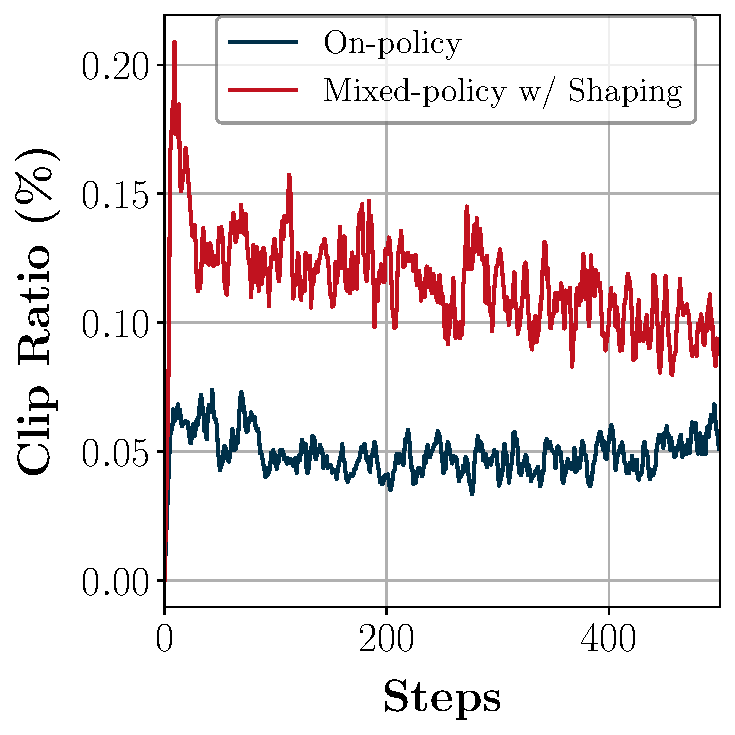
\includegraphics[width=\linewidth]{figs/clip_ratio.pdf}
%   % \vspace{-10pt}
%   \caption{\textbf{Ratio of clipped signals.}}
%   \label{fig:clip}
%   \vspace{-20pt}
% \end{wrapfigure}

% \begin{wrapfigure}{r}{0.3\textwidth}
%   \centering
%   \vspace{-40pt}
%   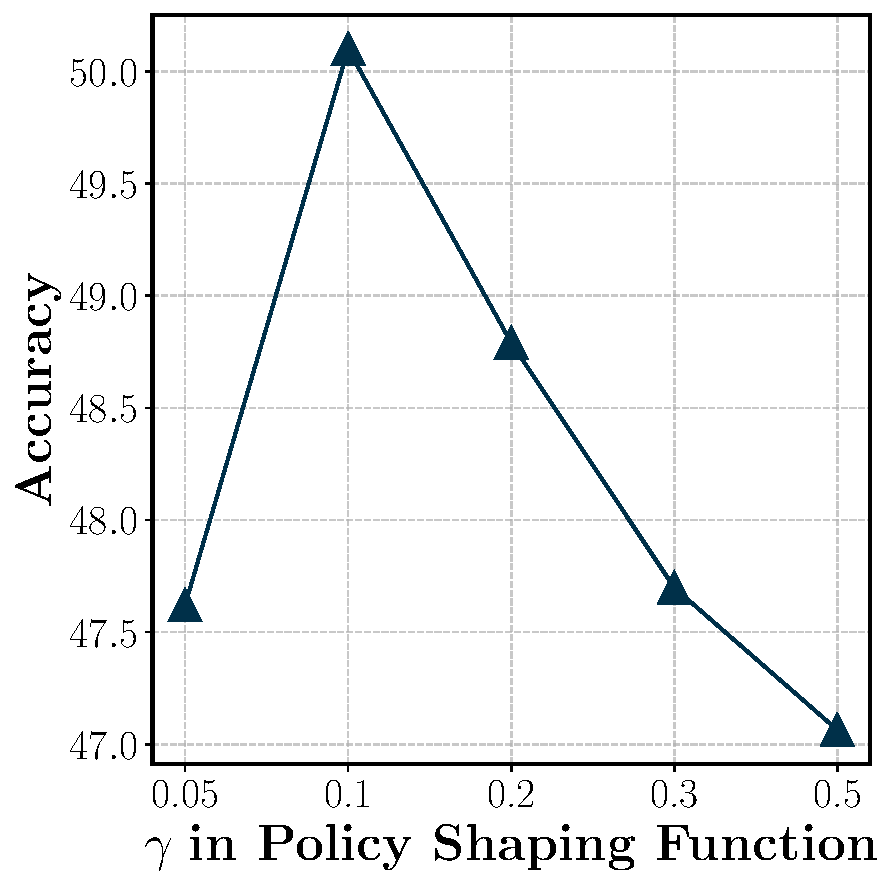
\includegraphics[width=\linewidth]{figs/gamma.pdf}
%   \vspace{-15pt}
%   \caption{\textbf{Accuracy versus the choice of $\gamma$.}}
%   \label{fig:gamma}
%   \vspace{-40pt}
% \end{wrapfigure}
\begin{wrapfigure}{r}{0.4\textwidth}
  \centering
  \vspace{-40pt}
  \begin{minipage}{\linewidth}
    \centering
    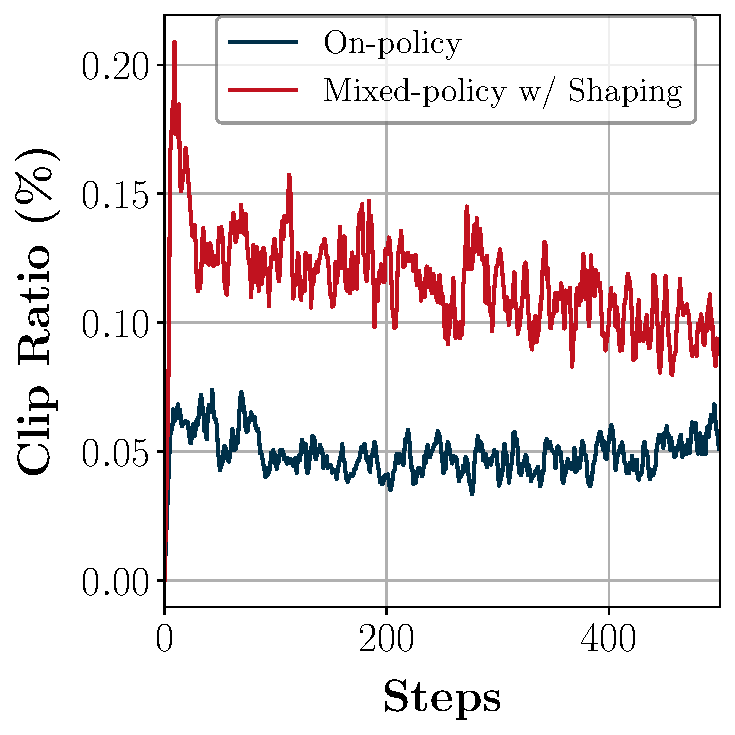
\includegraphics[width=\linewidth]{figs/clip_ratio.pdf}
    \caption{\textbf{Ratio of clipped signals.}}
    \label{fig:clip}
    \vspace{10pt}
    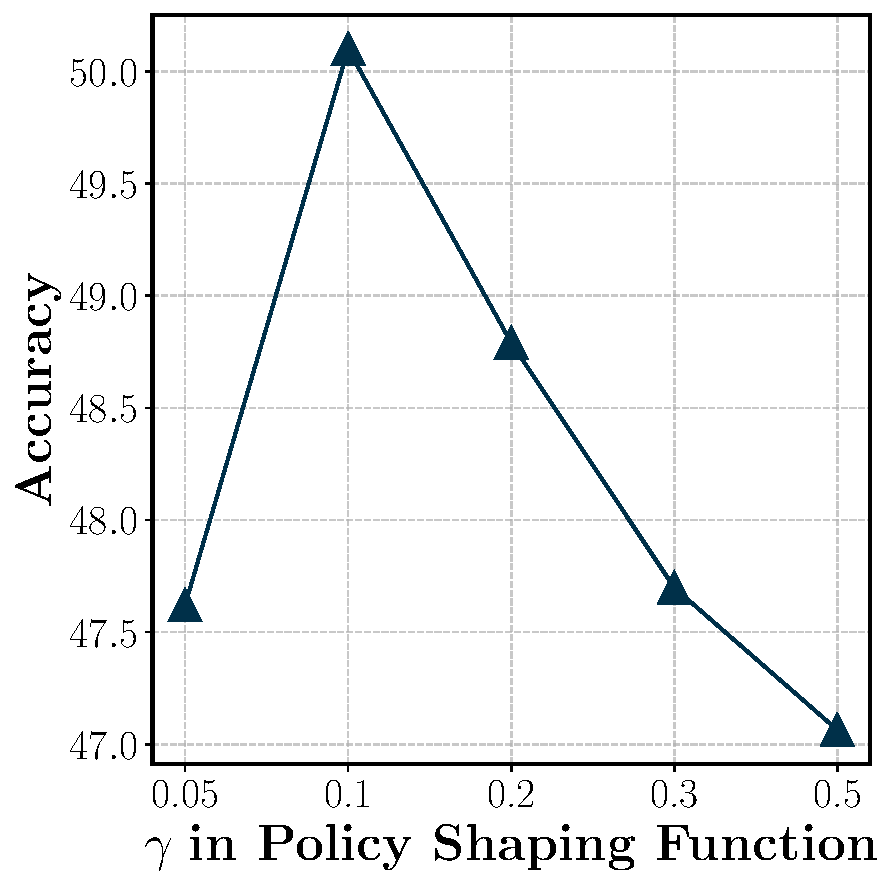
\includegraphics[width=\linewidth]{figs/gamma.pdf}
    \caption{\textbf{Accuracy versus the choice of $\gamma$.}}
    \vspace{-40pt}
    \label{fig:gamma}
  \end{minipage}
\end{wrapfigure}
% \vspace{-10pt}


% Another interesting effect we notice is that 
The clipping mechanism is introduced to constrain policy updates within a trust region~\cite{trpo}, thereby ensuring stable training. 
However, when incorporating off-policy guidance, the target behavior may deviate significantly from the model's current policy, especially early in training. 

As shown in Figure~\ref{fig:clip}, \m{LUFFY} experiences more frequent clipping compared to \m{On-Policy RL}, which can suppress learning from high-quality off-policy traces. 
To address this, we remove the on-policy clip to allow greater flexibility in updating toward unfamiliar yet effective actions, thereby unlocking the model's capacity to better integrate off-policy reasoning behaviors.


% \subsection{Importance Sampling for correcting the Gradient Computations}
% \begin{equation}\label{iw_pg}
%     \begin{gathered}
%     \nabla_{\theta} \mathcal{J}(\theta) = \mathbb{E}_{{\color{red}\tau_j \sim \pi_{\theta}(\tau)}} \left[ \nabla_{\theta} \log \pi_{\theta}(\tau_j) \hat{A_j} \right] \\
%     = \mathbb{E}_{\color{blue}\tau_j \sim \pi_{\phi}(\tau)} \left[ \frac{\pi_{\theta}(\tau_j)}{\pi_{\phi}(\tau_j)} \nabla_{\theta} \log \pi_{\theta}(\tau_j) \hat{A_j} \right].
% \end{gathered}
% \end{equation} 
% The importance sampling term effectively corrects the gradient from expectation of $\pi_{\theta}$~(red) to $\pi_{\phi}$~(blue). 


% \begin{table}[t]
% \centering
% \caption{Overall performance on six competition-level benchmark performance on Qwen2.5-Math-1.5B and Qwen2.5-Instruct-7B.}
% \label{tab:main_other_models}
% \resizebox{\textwidth}{!}{
% \begin{tabular}{lccccccc}
% \toprule
% \textbf{Model}                      & \textbf{AIME 24} & \textbf{AIME 25} & \textbf{AMC} & \textbf{MATH-500} & \textbf{Minerva} & \textbf{Olympiad} & \textbf{Avg.}  \\
% \midrule
% \multicolumn{8}{c}{\textit{Qwen2.5-Math-1.5B}} \\
% \midrule
% Qwen2.5-Math-1.5B-Base~\cite{qwen2.5_math}          & 7.9           & 4.7           & 26.4          & 31.0          & 12.1          & 21.5          & 17.3          \\
% Qwen2.5-Math-1.5B-Instruct~\cite{qwen2.5_math} & 11.4          & 8.5           & 47.4          & 75.2          & 27.6          & 38.7          & 34.8          \\\midrule
% SFT              & 15.2          & \textbf{14.3} & 43.5          & 74.8          & \textbf{30.9} & 36.9          & 40.3          \\
% On-Policy RL     & 12.6          & 6.5           & 42.6          & 68.8          & 22.1          & 34.4          & 36.1          \\
% LUFFY            & \textbf{15.2} & 12.7          & \textbf{46.8} & \textbf{79.4} & 26.5          & \textbf{42.4} & \textbf{42.1} \\
% % Qwen2.5-Math-1.5B          & 6.5    & 27.9 & 36.0    & 8.5    & 21.2    & 20.0 \\
% % Qwen2.5-Math-1.5B-Instruct & 11.8   & \textbf{47.5} & 75.8    & 27.9   & 39.9    & 40.6 \\
% % \midrule
% % SFT                        & 12.7   & 43.3 & 73.8    & 25.4   & 39.1    & 38.9 \\
% % On-policy RL                         & 11.6   & 42.2 & 69.6    & 22.1   & 35.0    & 36.1 \\
% % LUFFY                       & \textbf{16.5}   & 47.0 & \textbf{78.8}    & \textbf{28.3}   & \textbf{40.9}    & \textbf{42.3} \\
% \midrule
% \multicolumn{8}{c}{\textit{Qwen2.5-Instruct-7B}} \\
% \midrule
% Qwen2.5-7B-Instruct~\cite{qwen2.5} & 11.9 & 7.6 & 44.1 & 74.6 & 30.5 & 39.7 & 34.7 \\\midrule
% SFT          & 9.7  & 11.3 & 41.8 & 71.2 & 26.8 & 38.1 & 33.1 \\
% On-Policy RL & 16.5 & 10.7 & 47.5 & 75.8 & 35.3 & 41.9 & 37.9 \\
% LUFFY        & \textbf{16.6} & \textbf{15.7} & \textbf{52.2} & \textbf{81.4} & \textbf{36.8} & \textbf{48.7} & \textbf{41.9} \\\bottomrule
% % SFT  & 9.7  & 41.8 & 26.8 & 38.1 & 71.2 & 37.5 \\
% % On-policy RL  & 16.5 & 47.5 & 35.3 & 41.9 & 75.8 & 43.4 \\
% % LUFFY & \textbf{16.6} & \textbf{52.2} & \textbf{36.8} & \textbf{48.7} & \textbf{81.4} & \textbf{47.1}\\\bottomrule
% \end{tabular}}
% \end{table}









\subsection{Extension to More Models}
\label{app:more_models}

\begin{table}[t]
\centering
\caption{Overall performance on six competition-level benchmark performance on Qwen2.5-Math-1.5B, Qwen2.5-Instruct-7B and LLaMA-3.1-8B.}
\label{tab:main_other_models}
\resizebox{\textwidth}{!}{
\begin{tabular}{lccccccc}
\toprule
\textbf{Model}                      & \textbf{AIME 24} & \textbf{AIME 25} & \textbf{AMC} & \textbf{MATH-500} & \textbf{Minerva} & \textbf{Olympiad} & \textbf{Avg.}  \\
\midrule
\normalrow
\multicolumn{8}{c}{\textit{Qwen2.5-Math-1.5B}} \\
\midrule
Qwen2.5-Math-1.5B-Base~\cite{qwen2.5_math} & 7.2  & 3.6  & 26.4 & 28.0 & 9.6  & 21.2 & 16.0 \\
Qwen2.5-Math-1.5B-Instruct~\cite{qwen2.5_math} & 12.1 & 8.9  & 48.1 & 77.4 & 28.7 & 39.1 & 35.7 \\\midrule
SFT & 11.7 & \textbf{13.2} & 37.8 & 70.6 & 26.8 & 31.3 & 31.9 \\
On-Policy RL & 11.8 & 7.7  & 40.2 & 61.8 & 26.8 & 32.0 & 30.0 \\
LUFFY & \textbf{16.0} & 13.1 & \textbf{47.1} & \textbf{80.2} & \textbf{30.5} & \textbf{41.0} & \textbf{38.0} \\
% Qwen2.5-Math-1.5B-Base~\cite{qwen2.5_math}          & 7.9           & 4.7           & 26.4          & 31.0          & 12.1          & 21.5          & 17.3          \\
% Qwen2.5-Math-1.5B-Instruct~\cite{qwen2.5_math} & 11.4          & 8.5           & 47.4          & 75.2          & 27.6          & 38.7          & 34.8          \\\midrule
% SFT              & 15.2          & \textbf{14.3} & 43.5          & 74.8          & \textbf{30.9} & 36.9          & 40.3          \\
% On-Policy RL     & 12.6          & 6.5           & 42.6          & 68.8          & 22.1          & 34.4          & 36.1          \\
% LUFFY            & \textbf{15.2} & 12.7          & \textbf{46.8} & \textbf{79.4} & 26.5          & \textbf{42.4} & \textbf{42.1} \\
% Qwen2.5-Math-1.5B          & 6.5    & 27.9 & 36.0    & 8.5    & 21.2    & 20.0 \\
% Qwen2.5-Math-1.5B-Instruct & 11.8   & \textbf{47.5} & 75.8    & 27.9   & 39.9    & 40.6 \\
% \midrule
% SFT                        & 12.7   & 43.3 & 73.8    & 25.4   & 39.1    & 38.9 \\
% On-policy RL                         & 11.6   & 42.2 & 69.6    & 22.1   & 35.0    & 36.1 \\
% LUFFY                       & \textbf{16.5}   & 47.0 & \textbf{78.8}    & \textbf{28.3}   & \textbf{40.9}    & \textbf{42.3} \\
\midrule
\normalrow
\multicolumn{8}{c}{\textit{Qwen2.5-Instruct-7B}} \\
\midrule
 Qwen2.5-7B-Instruct~\cite{qwen2.5} & 11.7 & 7.5  & 43.8 & 71.8 & 30.9 & 40.4 & 34.4 \\\midrule
SFT & 7.9  & 9.2  & 36.0 & 68.6 & 21.3 & 31.1 & 29.0 \\
On-Policy RL &14.1 & 8.3  & 43.5 & 74.0 & \textbf{33.8} & 37.6 & 35.2 \\
LUFFY & \textbf{17.7} & \textbf{14.8} & \textbf{50.9} & \textbf{82.0} & 31.3 & \textbf{47.4} & \textbf{40.7} \\
% Qwen2.5-7B-Instruct~\cite{qwen2.5} & 11.9 & 7.6 & 44.1 & 74.6 & 30.5 & 39.7 & 34.7 \\\midrule
% SFT          & 9.7  & 11.3 & 41.8 & 71.2 & 26.8 & 38.1 & 33.1 \\
% On-Policy RL & 16.5 & 10.7 & 47.5 & 75.8 & 35.3 & 41.9 & 37.9 \\
% LUFFY        & \textbf{16.6} & \textbf{15.7} & \textbf{52.2} & \textbf{81.4} & \textbf{36.8} & \textbf{48.7} & \textbf{41.9} \\
\midrule
\normalrow
\multicolumn{8}{c}{\textit{LLaMA-3.1-8B}} \\
\midrule
LLaMA-3.1-8B-Instruct~\cite{llama3} & 5.1 & 0.4 & 18.6 & 44.6 & 19.5 & 14.1 & 17.1 \\\midrule
SFT & 0.5 & 0.1 & 5.4  & 20.2 & 4.0  & 5.3  & 5.9  \\
On-Policy RL & 0.3 & \textbf{0.5} & 9.4  & 23.4 & \textbf{17.6} & 6.1  & 9.6  \\
LUFFY & \textbf{1.9} & 0.1 & \textbf{13.5} & \textbf{39.0} & 15.1 & \textbf{9.6} & \textbf{13.2}\\\bottomrule
\end{tabular}}
\end{table}

% \jianhao{todo: modify}
% To assess the general applicability of our method, we extend \m{LUFFY} to a smaller base model: Qwen2.5-Math-1.5B. 
% We also consider Qwen2.5-Instruct-7B to validate LUFFY on non-zero RL paradigm, i.e., RL on Instruction-tuned models. 
Table~\ref{tab:main_other_models} presents the detailed performance across six challenging competition-level benchmarks for Qwen2.5-Math-1.5B, Qwen2.5-Instruct-7B, and LLaMA-3.1-8B.
On all three models, \m{LUFFY} achieves consistent and substantial improvements, surpassing both \m{SFT} and \m{On-Policy RL}. 
On Qwen2.5-Math-1.5B, \m{LUFFY} attains an average score of \textbf{38.0}, demonstrating notable gains of +6.1 and +8.0 points over \m{SFT} and \m{On-Policy RL}, respectively. 
Similar advantages are observed on the Qwen2.5-Instruct-7B and LLaMA-3.1-8B, where \m{LUFFY} consistently outperforms baselines across all benchmarks. 
% Particularly, it achieves an overall score of \textbf{41.9}, representing clear improvements of +8.8 points over \m{SFT} and +4.0 points compared with \m{On-Policy RL}.



\subsection{Ablation Study}
In this section, we perform an ablation study to examine the contributions of \m{LUFFY} components, as summarized in Table~\ref{tab:ablate}. 
Shaping and NoClip both positively contribute to the final performance of Mixed-Policy training.
However, applying these enhancements without off-policy guidance (On-Policy + No Clip/Shaping) does not yield improvement, underscoring the necessity of external signals to acquire nuanced and generalizable reasoning skills.

\begin{table}[t]
\centering
\caption{Ablation study on LUFFY components.}
\label{tab:ablate}
\resizebox{\textwidth}{!}{
\begin{tabular}{lccccccc}
\toprule
\textbf{Model} & \textbf{AIME 24}& \textbf{AIME 25} & \textbf{AMC} & \textbf{MATH-500} & \textbf{Minerva} & \textbf{Olympiad} & \textbf{Avg.}  \\
\midrule
% Mixed-Policy RL      & 19.2 & 58.7 & 83.8 & 30.9 & 49.9 & 48.5 \\
% ~~~ + Shaping           & 30.0 & 61.7 & 86.2 & 36.4 & 55.6 & 54.0 \\
% ~~~ + Shaping + NoClip (LUFFY) & 29.5 & 66.1 & 88.4 & 33.8 & 56.4 & \textbf{54.9} 
% Mixed-Policy RL      & 19.2 & 16.9 & 58.7 & 83.8 & 30.9 & 49.9 & 43.2 \\
% ~~~ + Shaping           & 30.0 & 22.6 & 61.7 & 86.2 & 36.4 & 55.6 & 48.7 \\
% ~~~ + Shaping + NoClip & 29.5 & 23.2 & 66.1 & 88.4 & 33.8 & 56.4 & 49.6 \\\midrule
% On-Policy RL           & 24.6 & 15.7 & 61.3 & 84.6 & 34.9 & 47.9 & 44.8 \\
% ~~~ + Shaping & 21.8 & 14.7 & 57.6 & 81.6 & 33.5 & 44.6 & 42.3 \\
% ~~~ + No Clip & 22.7 & 17.3 & 61.6 & 83.4 & 34.9 & 50.7 & 45.1 
Mixed-Policy RL & 19.4 & 17.7 & 58.9 & 84.6 & 35.7 & 49.9 & 44.4 \\
~~~ + Shaping & 27.4 & 21.7 & 61.2 & 86.6 & 37.1 & 53.0 & 47.8 \\
~~~ + Shaping + NoClip & 29.4 & 23.1 & 65.6 & 87.6 & 37.5 & 57.2 & 50.1 \\\midrule
On-Policy RL &25.1 & 15.3 & 62.0 & 84.4 & 39.3 & 46.8 & 45.5 \\
~~~ + Shaping & 21.3 & 13.6 & 58.0 & 80.6 & 36.8 & 41.8 & 42.0 \\
~~~ + No Clip & 21.5 & 17.4 & 61.1 & 83.4 & 36.8 & 49.0 & 44.9
\\\bottomrule
\end{tabular}}
\end{table}


\subsection{Hyperparameter Study}
\label{app:hyper_study}

In this section, we study the choice of $\gamma$ in policy shaping function. The results are shown in Figure \ref{fig:gamma}, trained from Qwen2.5-Math-7B. We choose $\gamma$ value from [0.05, 0.1, 0.2, 0.3, 0.5].
When $\gamma=0.1$, the model performs the best with 50.1 accuracy scores, and increasing or decreasing this value leads to a notable decline in model performance. Therefore, we consistently use $\gamma=0.1$ throughout our experiments.





\section{Analysis}
\label{app:analysis}

\begin{wrapfigure}{r}{0.48\textwidth}
  \centering
  \vspace{-30pt}
  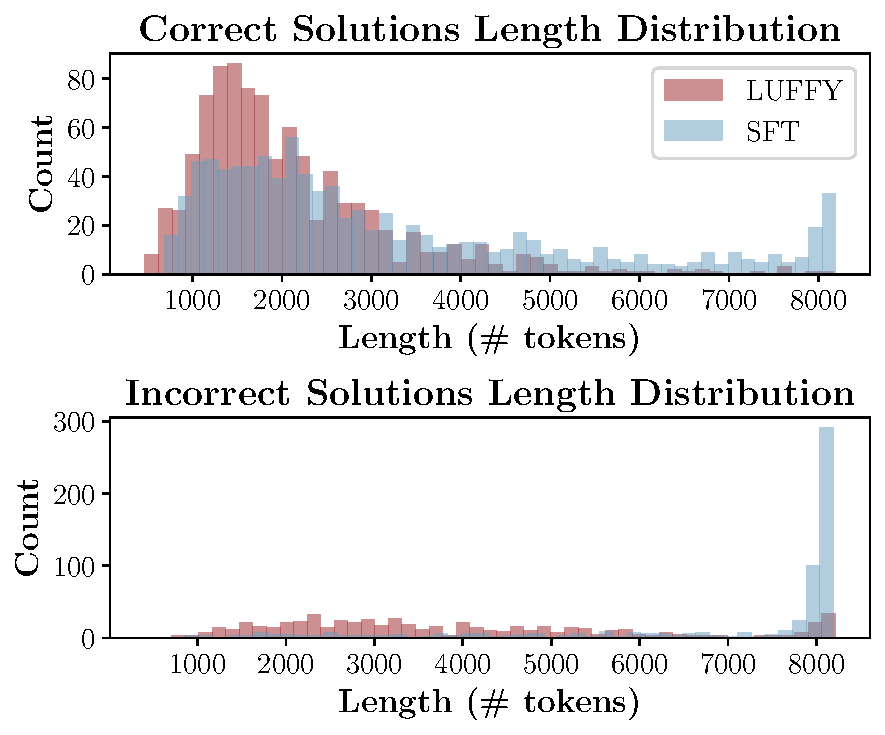
\includegraphics[width=\linewidth]{figs/length_dist.pdf}
  \vspace{-15pt}
  \caption{\textbf{Generation length of correct and incorrect solutions.}}
  \label{fig:length}
  \vspace{-30pt}
\end{wrapfigure}



In this section, we analyze how \m{LUFFY} effectively leverages off-policy guidance, i.e., \textit{imitating to illuminate}, to improve reasoning quality and generalization.


\subsection{LUFFY Learns Strategically from Off-Policy Traces, While SFT Imitates Rigidly}
\label{app:bleu}




% \paragraph{LUFFY Selectively Learns Off-policy Traces.}

% % Beyond generation length, imitation behavior can also be observed through the similarity between model outputs and off-policy traces. 
% Imitation behavior can be observed through the similarity between model outputs and off-policy traces. 
% To quantify this, we compare generations from \m{SFT}, \m{On-Policy RL}, and \m{LUFFY} against those from DeepSeek-R1 on a held-out set of 1,000 samples, using BLEU~\cite{papineni-etal-2002-bleu} as the similarity metric. 
% The resulting BLEU scores are 57.5 for \m{SFT}, 8.8 for \m{On-Policy RL}, and 44.8 for \m{LUFFY}, reflecting the strong imitation behavior of \m{SFT} and the more selective, yet substantial, imitation in \m{LUFFY}.



% \subsection{LUFFY Learns Off-policy Traces More Effectively.}

\label{app:effective_reasoning}
We compare the generation length distributions of \m{LUFFY} and \m{SFT} on the combined set of six mathematical reasoning benchmarks. 
As shown in Figure~\ref{fig:length}, \m{LUFFY} produces significantly shorter generations on average (2,832 tokens) compared to \m{SFT} (4,646 tokens), suggesting a more effective reasoning process that balances imitation and exploration. 
This observation helps explain the excessive training costs of methods that naively combine SFT and RL, e.g., \m{SFT+RL} and \m{RL w/ SFT Loss} (Table~\ref{tab:comparision}), as these models spend substantially more compute on producing unnecessarily lengthy CoTs during the RL roll-out stage.
In contrast, \m{SFT} often mimics the surface form of off-policy demonstrations without genuinely engaging in problem-solving. 
This behavior is especially evident in incorrect outputs, where \m{SFT} frequently generates overly long and ultimately unproductive reasoning traces. 
These results indicate that while both methods are exposed to similar off-policy signals, \m{LUFFY} learns to selectively internalize useful reasoning patterns, whereas \m{SFT} tends to overfit to superficial features of the off-policy data. 

\begin{wrapfigure}{r}{0.4\textwidth}
  \centering
  % \vspace{-10pt}
  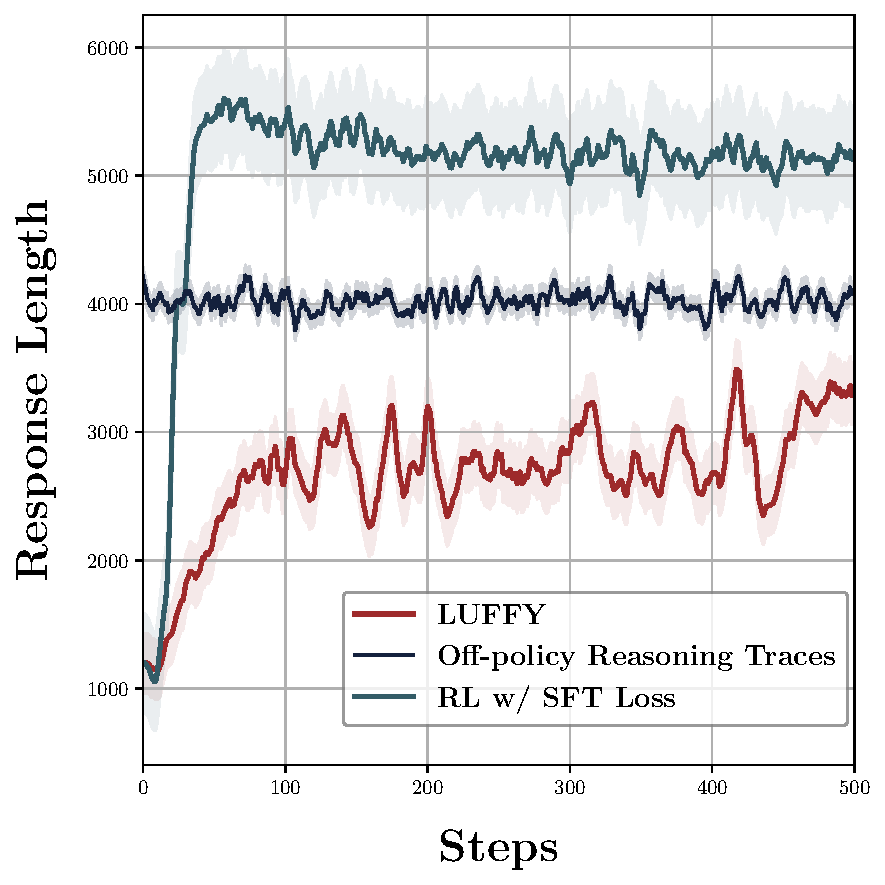
\includegraphics[width=\linewidth]{figs/compare_multi_sft_rl_length.pdf}
  % \vspace{-20pt}
  \caption{Generation length of \m{RL w/ SFT Loss} and \m{LUFFY}.}
  \label{fig:compare_multi}
  \vspace{-10pt}
\end{wrapfigure}



We further analyze the generation lengths of \m{RL w/ SFT Loss} and \m{LUFFY} during training, as shown in Figure~\ref{fig:compare_multi}.
\m{RL w/ SFT Loss} quickly imitates the off-policy traces, exhibiting a steep increase in generation length early in training.
However, it soon becomes trapped in the superficial patterns of the demonstrations, leading to excessively long outputs that even surpass the length of the original off-policy traces.
In contrast, \m{LUFFY}'s dynamic advantage balancing between on-policy and off-policy rollouts encourages more strategic learning. 
As a result, its generation length grows more gradually and steadily, reflecting a more selective and grounded adoption of reasoning behavior.

\begin{wrapfigure}{r}{0.4\textwidth}
  \centering
  % \vspace{-12pt}
  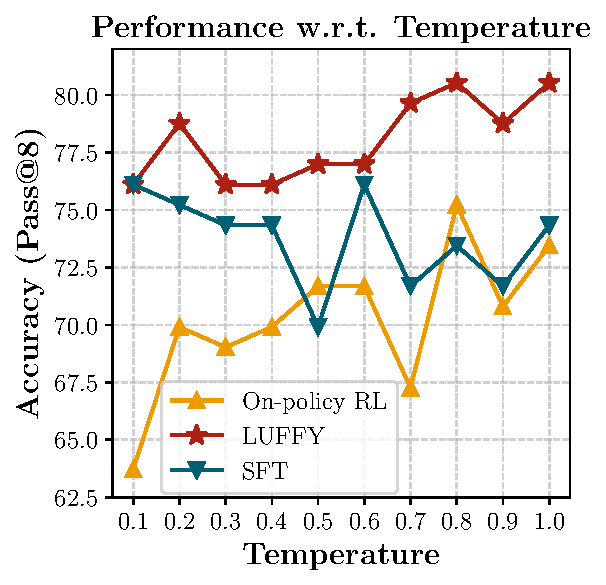
\includegraphics[width=\linewidth]{figs/temp.pdf}
  \caption{\textbf{Pass@8 accuracy (on the merge sets of AIME 2024 and AMC) under different generation temperatures.}}
  \label{fig:temp}
\end{wrapfigure}

Beyond generation length, imitation behavior can also be observed through the similarity between model outputs and off-policy traces. 
To quantify this, we compare generations from \m{SFT}, \m{On-Policy RL}, and \m{LUFFY} against those from DeepSeek-R1 on a held-out set of 1,000 samples, using BLEU~\cite{papineni-etal-2002-bleu} as the similarity metric. 
The resulting BLEU scores are 57.5 for \m{SFT}, 8.8 for \m{On-Policy RL}, and 44.8 for \m{LUFFY}, reflecting the strong imitation behavior of \m{SFT} and the more selective, yet substantial, imitation in \m{LUFFY}.
We present a case study in Appendix~\ref{app:case}. 
% bleu
% average length: 2832 v.s. 4646
% onp average bleu score: 0.0875382039230854
% ours average bleu score: 0.44787132916101197
% sft average bleu score: 0.575403136883539



% \textbf{\m{LUFFY} has the potential to scale test-time while SFT cannot. } 
\subsection{LUFFY Can Explore During Test-time While SFT Cannot. }
\label{app:better_exploration}

We compute pass@8 accuracy on the combined AIME 2024 and AMC datasets, varying the generation temperature from 0.1 to 1.0. 
As shown in Figure~\ref{fig:temp}, both RL-based methods (\m{On-Policy RL} and \m{LUFFY}) exhibit strong exploratory capabilities, with pass@8 improving as the temperature increases, showing potential in scaling test-time compute~\cite{setlur2025scaling}. 
In contrast, although \m{SFT} performs comparably to \m{LUFFY} under near-deterministic decoding (temperature 0.1), its performance deteriorates at higher temperatures, failing to uncover additional correct reasoning paths. 
This highlights the fragility and limited adaptability of \m{SFT}, 
which aligns with prior findings~\cite{chu2025sftmemorizesrlgeneralizes,vl-thinking2025} that suggest SFT tends to memorize reasoning patterns rather than learning generalizable reasoning capability.

